\section{实验三\ VGA 与串行端口}

\subsection{实验目的}

\begin{enumerate}
    \item 了解 Linux 中 VGA 的实现,掌握 printk 等字符打印函数的实现方法。
    \item 了解 Linux 通过串行端口与终端交换信息的函数实现。
\end{enumerate}

\textbf{视频图形阵列}(Video Graphics Array,简称 VGA)是 IBM 于 1987 年提出的一种电脑显示标准。运用该标准的接口被称为 VGA 端子,通常用于在电脑的显示卡、显示器及其他设备发送模拟信号。本次实验关注于内核对彩色字符模式显示缓冲区的控制。

\subsection{80 * 25 彩色字符模式显示缓冲区的结构}

内存地址中,B8000h $\backslash$ BFFFFh 共 32KB 的空间,是 80*25 彩色字符模式的显示缓冲区。在这个地址空间中写入数据,写入的内容会立即出现在显示器上。

在 80*25 彩色字符模式下,显示器可显示 25 行,每行 80 个字符,每个字符可以有 256种属性,包括背景色、前景色(即字体色)、闪烁、高亮等组合而成的属性。

一个字符在显示缓冲区中占用 2 个字节,分别存放其 ASCII 码和属性。一屏的内容在显示缓冲区中共占用占 2 * 25 * 80 = 4000 字节。

显示缓冲区分 8 页,每页 4 KB,显示器可显示任意一页的内容。一般地,显示第 0 页内容,即显示 B8000H ~ B8F9FH 中的共 4000 字节的内容。

在一页显示缓冲区中,一行的 80 个字符占用 160 字节,偏移 000 ~ 09f 对应显示器上的第一行,偏移 0A0 ~ 13f 对应显示器上的第二行,以此类推。

在属性字节中,闪烁、背景色、高亮与前景色是按位设置的,如表 \ref{tab:属性字节中每位的具体含义}.

\begin{table}[]
\caption{属性字节中每位的具体含义}
\label{tab:属性字节中每位的具体含义}
\begin{tabular}{llllllll}
\hline
\multicolumn{1}{|l|}{7} & \multicolumn{1}{l|}{6} & \multicolumn{1}{l|}{5} & \multicolumn{1}{l|}{4} & \multicolumn{1}{l|}{3} & \multicolumn{1}{l|}{2} & \multicolumn{1}{l|}{1} & \multicolumn{1}{l|}{0} \\ \hline
\multicolumn{1}{|l|}{BL} & \multicolumn{1}{l|}{R} & \multicolumn{1}{l|}{G} & \multicolumn{1}{l|}{B} & \multicolumn{1}{l|}{I} & \multicolumn{1}{l|}{R} & \multicolumn{1}{l|}{G} & \multicolumn{1}{l|}{B} \\ \hline
\multicolumn{1}{|l|}{闪烁} & \multicolumn{1}{l|}{背景色} & \multicolumn{1}{l|}{背景色} & \multicolumn{1}{l|}{背景色} & \multicolumn{1}{l|}{高亮} & \multicolumn{1}{l|}{前景色} & \multicolumn{1}{l|}{前景色} & \multicolumn{1}{l|}{前景色} \\ \hline
 &  &  &  &  &  &  & 
\end{tabular}
\end{table}

下面介绍内核中用于 VGA 的一些函数。

\subsubsection{函数 video\_putchar\_at(char ch, int x, int y, char attr)}

本函数用于在屏幕指定位置 (x,y) 处输出指定字符串 ch,并且指定字符串 ch 后光标的颜色 attr. 其中,x 是行数,y 是列数。

ch 与 attr 变量不需要额外的处理,仅需要将这两个变量赋值到合适的内存地址处。

\subsubsection{不定参数函数}

在内核调用函数 printk 时,需要被格式化输出的内容长度是不定的,因此 printk 是一个不定参数函数。函数 printk 的实现中,将用到 <stdarg.h> 库中的数据结构或函数:va\_list、va\_start、va\_arg.\footnote{\url{https://msdn.microsoft.com/zh-cn/library/kb57fad8.aspx}}

\subsubsection{函数 printk(char *fmt, ...)}

printf 与 printk 在实现的功能上几乎一致,根据使用 C 语言函数 printf 的经验,可知这个格式化输出函数的首个参数 char *fmt 应当表示一段字符串的首位,以 *fmt 为首的字符串描述了格式化输出的格式。

这个字符串中可能含有以 “\%” 为首位的子串,表示一个数字、一个char类字符或一段字符串,它具体的值即 printk 的某个在 *fmt 之后的参数。

\begin{mdframed}[hidealllines=true,backgroundcolor=gray!20]
\textbf{练习 } 打开 exp3/kernel/printk.c,尝试依次实现 video\_putchar\_at 和 printk 函数。

首先,思考一个屏幕坐标(x, y)对应的显存地址是如何计算的?其中,显存地址的首位在 exp3/kernel/printk.c 中由 video\_buffer 指针表示。

请通过调用函数 printnum、video\_putchar、va\_start、va\_arg,尝试为函数 printk 实现如下功能\footnote{参考网站:\url{https://wiki.osdev.org/Printing_To_Screen}}:

\begin{enumerate}
    \item 字符串无 “\%” 时能直接在屏幕上输出字符串的内容
    \item 读取到 “\%d”,根据某个参数输出一个有符号十进制整数
    \item 读取到 “\%u”,根据某个参数输出一个无符号十进制整数
    \item 读取到 “\%x”,根据某个参数输出一个无符号十六进制整数
    \item 读取到 “\%c”,根据某个参数输出一个字符
    \item 读取到 “\%s”,根据某个参数输出一段字符串
    \item 读取到 “\%\%”,输出百分号“\%”
\end{enumerate}

注意,你需要仔细考虑各种状态转移。例如,你可能认为读取到 “\%” 时是解析一项参数的开始,但它同样可能是该字符串的最后一个字符,即一个百分号可能没有后继的字符。

若函数 video\_putchar\_at 与函数 printk 已成功实现,使用 QEMU 运行 neuos,将见到如图 \ref{fig:函数printk成功实现} 的界面。printk 函数是由 exp3/kernel/main.c 调用的。

\end{mdframed}

\begin{figure}[htbp]
    \centering
    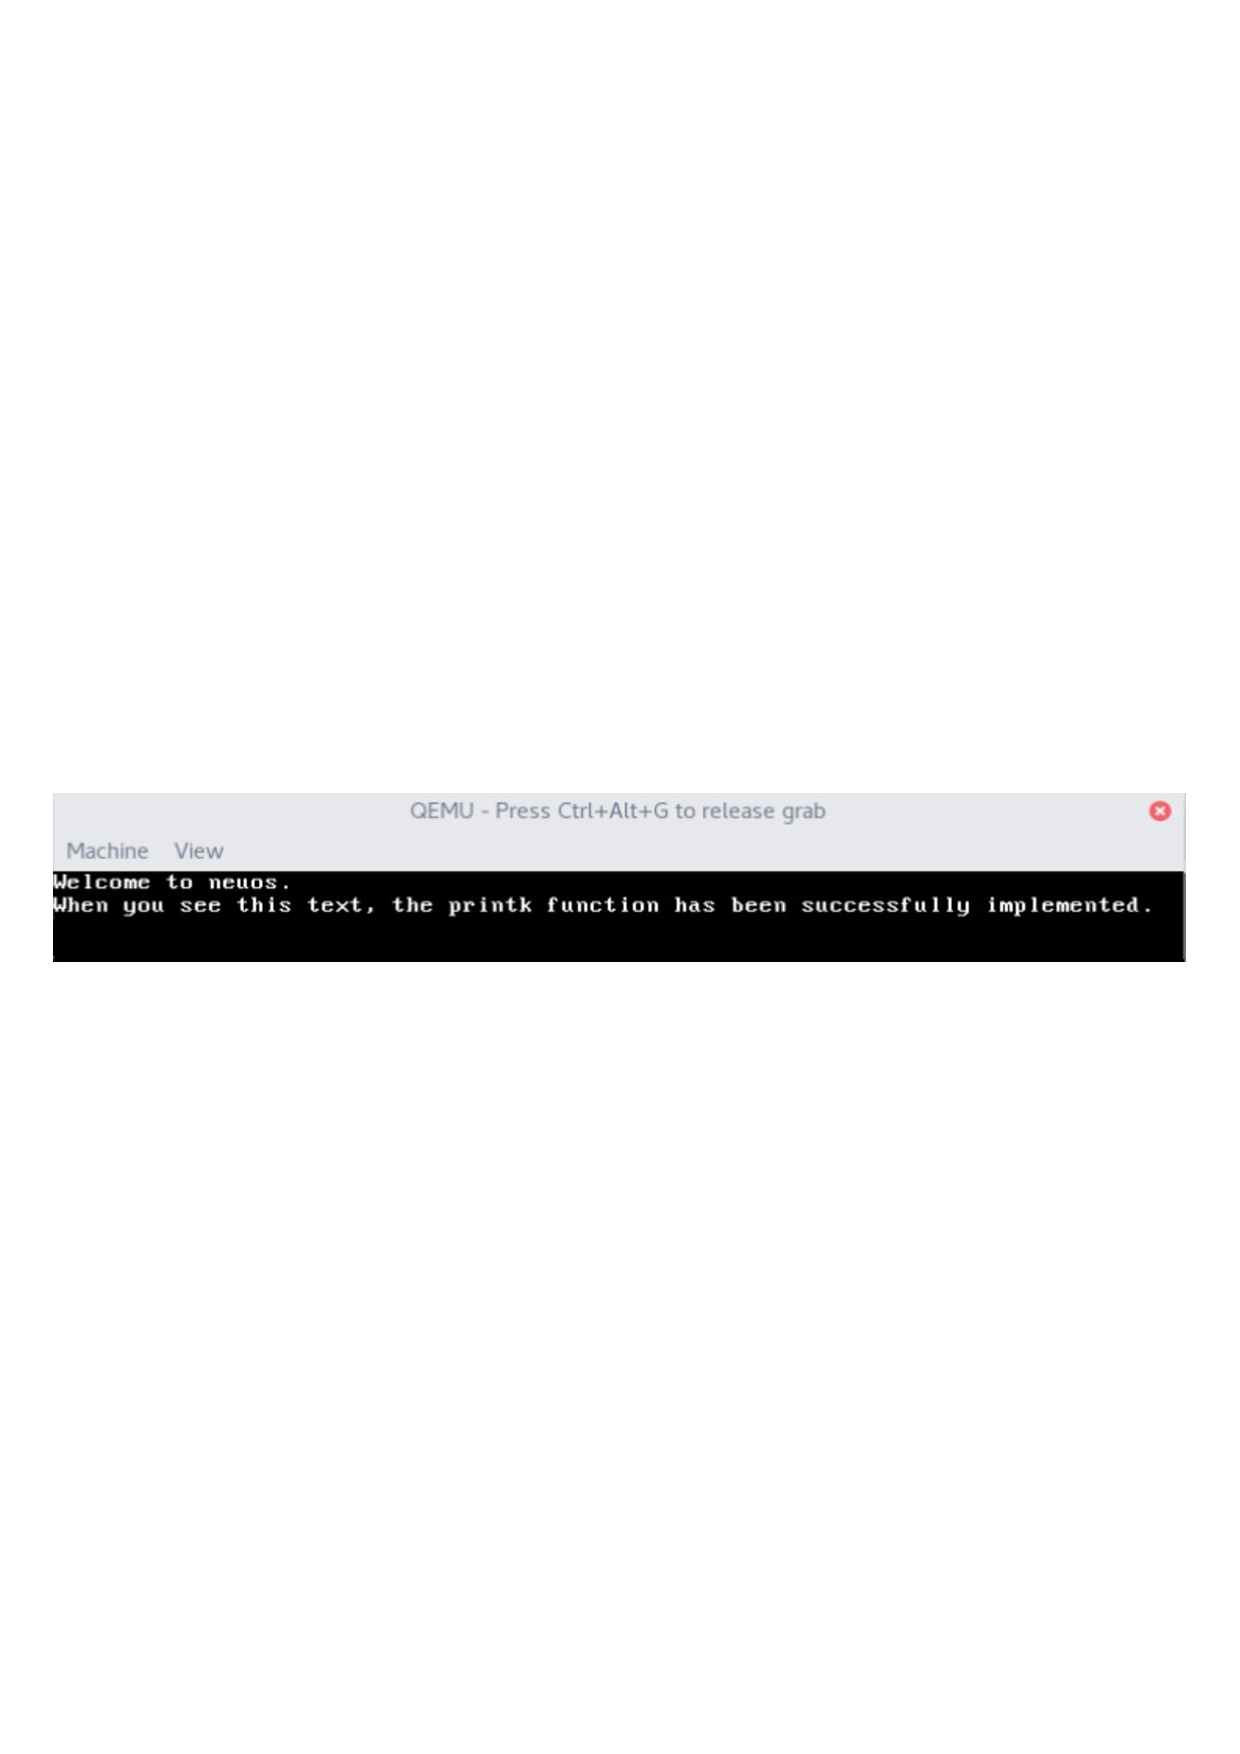
\includegraphics[width=\textwidth]{img/函数printk成功实现.pdf}
    \caption{函数 printk 成功实现}
    \label{fig:函数printk成功实现}
\end{figure}

\begin{mdframed}[hidealllines=true,backgroundcolor=gray!20]
\textbf{练习 }尝试通过调用 printk.c 中的两个函数 memcpy 与 video\_putchar\_at 实现滚屏函数 roll\_screen. 滚屏函数被调用的条件应当是,需要输出字符到当前屏幕的最后一行之后。因此需要将当前屏幕的内容整体上移,使得屏幕最后一行能够输出新的内容。

要验证函数 roll\_screen 是否成功实现,可打开目录 exp3/kernel/main.c,使用函数 printk 输出足够多的字符,再运行 neuos,测试能否成功滚屏。
\end{mdframed}

\subsection{串行端口}

\textbf{串行端口}(Serial port)主要用于串行式逐位数据传输。可用于连接外置调制解调器、打印机、路由器等设备。在消费电子领域已被 USB 替代,在网络设备中仍是主要的传输控制方式。

通过串行接口,Linux 设备,即使并非计算机,也可实现与其他设备的通信;本实验中的串行端口用于将 neuos 中的信息打印到 NEU-OS Lab Environment 的终端中。

\begin{mdframed}[hidealllines=true,backgroundcolor=gray!20]
\textbf{练习 }进入 exp3/kernel 目录,打开 serial.c 源文件。

函数 is\_transit\_empty 用于判断是否能够传输,若允许传输,函数返回 0.

结合函数 is\_transit\_empty 与端口输出函数 outb,实现函数 s\_putchar. 参考 Serial Ports - OSDev Wiki 4.3 节\footnote{\url{http://wiki.osdev.org/Serial_Ports}}。

然后,类似于 printk 函数的实现,请通过调用函数 s\_printnum、s\_putchar、va\_start、va\_arg,尝试为函数 s\_printk 实现如下功能:

\begin{enumerate}
    \item 字符串无 “\%” 时能直接在屏幕上输出字符串的内容
    \item 读取到 “\%d”,根据某个参数输出一个有符号十进制整数
    \item 读取到 “\%u”,根据某个参数输出一个无符号十进制整数
    \item 读取到 “\%x”,根据某个参数输出一个无符号十六进制整数
    \item 读取到 “\%c”,根据某个参数输出一个字符
    \item 读取到 “\%s”,根据某个参数输出一段字符串
    \item 读取到 “\%\%”,输出百分号“\%”
\end{enumerate}

若函数 s\_putchar 与函数 s\_printk 已成功实现,使用 QEMU 运行 neuos,运行结果如图 \ref{fig:函数sprintk成功实现} 所示,字符被输出到 os 的终端而不是 QEMU 界面中。

\end{mdframed}

\begin{figure}[htbp]
    \centering
    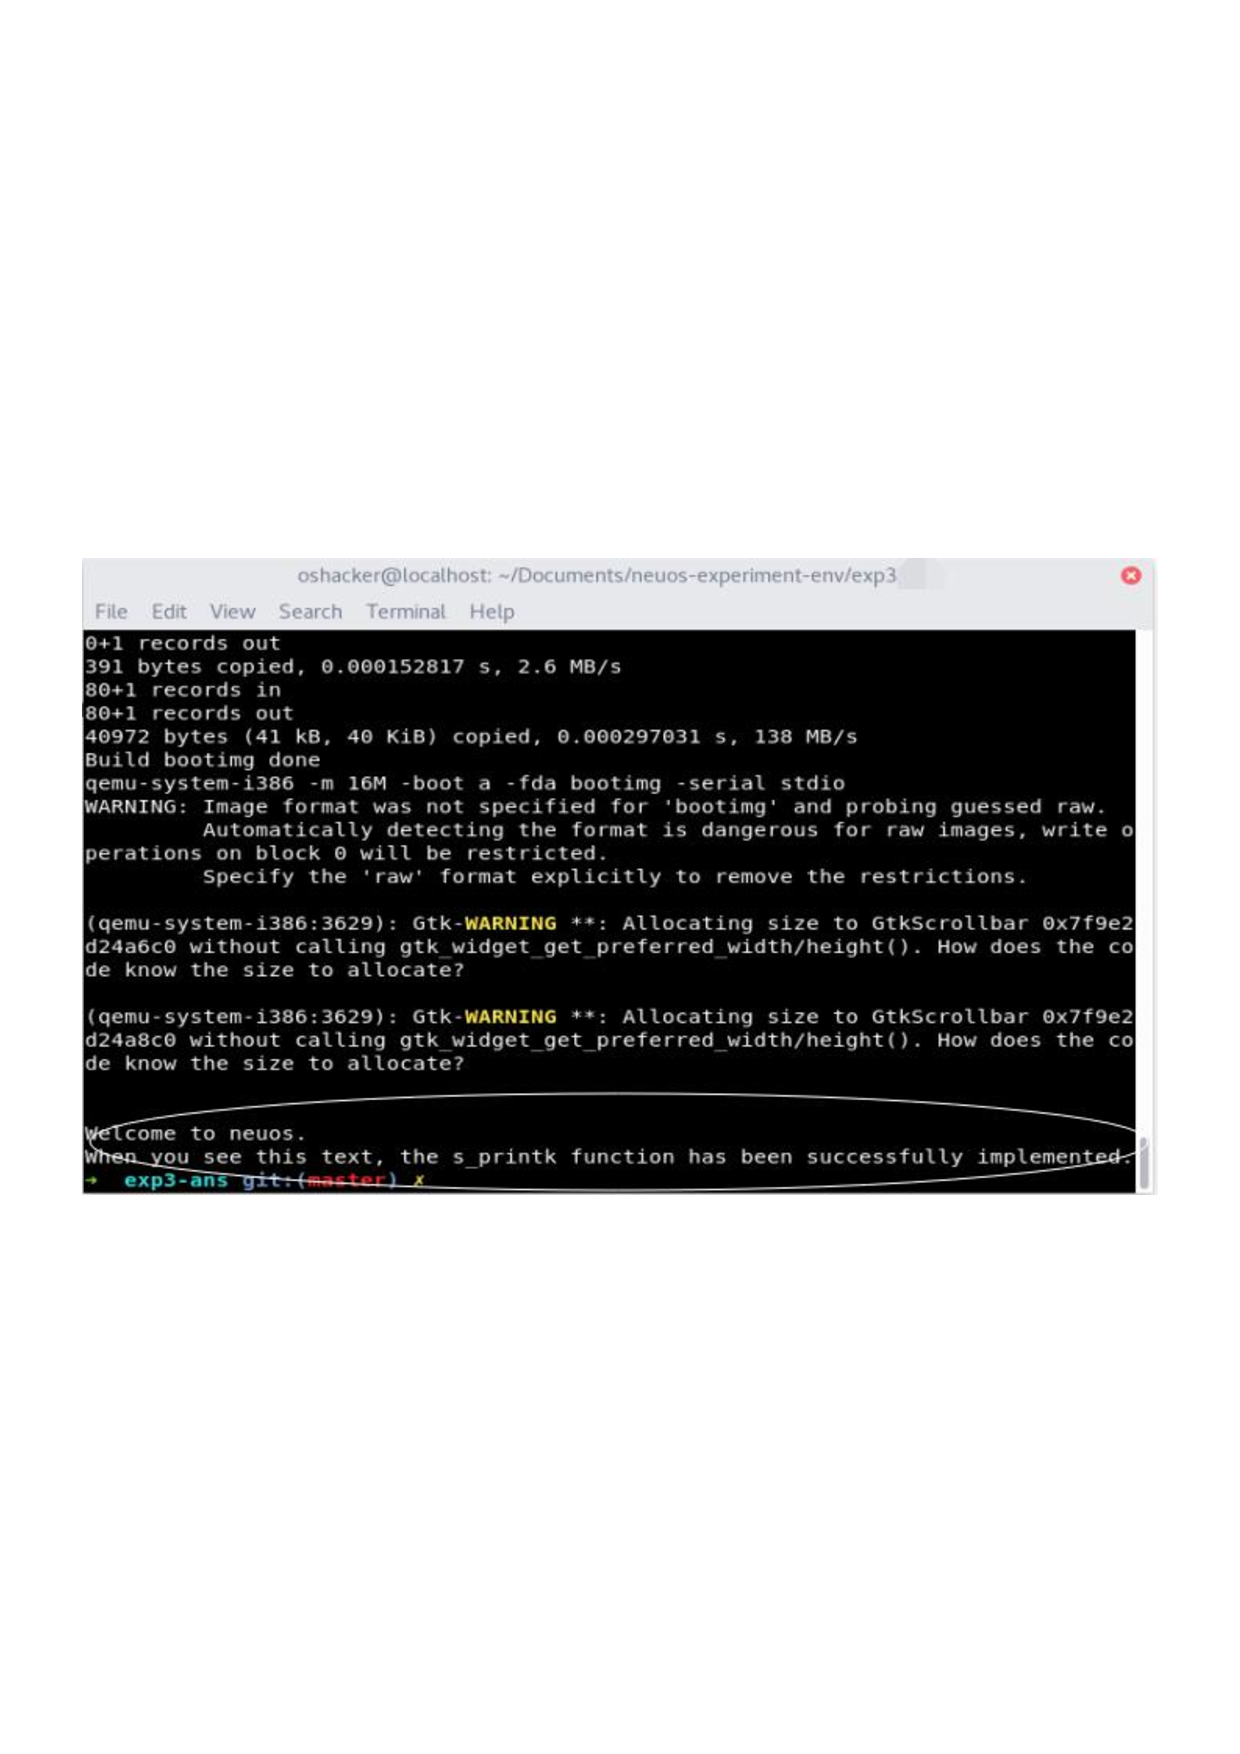
\includegraphics[width=\textwidth]{img/函数s_printk成功实现.pdf}
    \caption{函数 s\_printk 成功实现}
    \label{fig:函数sprintk成功实现}
\end{figure}

\begin{mdframed}[hidealllines=true,backgroundcolor=gray!20]
\textbf{练习 }在 exp3/kernel/serial.c 源文件的末尾,尝试实现通过串行端口读取信息的代码。仅尝试完成代码\footnote{参考 \url{http://wiki.osdev.org/Serial_Ports} 读取数据部分。},不必实现最终效果。
\end{mdframed}

\begin{mdframed}[hidealllines=true,backgroundcolor=gray!20]
\textbf{拓展学习 }找到 printk.c 源文件 208 行以后的“拓展学习”部分,实现具有指定 8 种颜色功能的函数 echo;echo 需要调用 video\_putchar\_color 等函数。

实现效果参考 \url{http://misc.flogisoft.com/bash/tip_colors_and_formatting},考虑到实现的难度等因素,以下描述与该参考网站的描述并不完全一致。

例如,echo(“$\backslash$033[x;ymneuos”); 可将 “neuos” 以 x 为前景色,y 为背景色输出。其中 x 和 y 是两个数字,均是 0\textasciitilde7 的整数,其表示的颜色见表 \ref{tab:前景色与背景色代码表示的颜色}。m 作为颜色的唯一后缀。

如果没有 “$\backslash$033[” 指定颜色,函数 echo 应直接输出文本。这个格式是严格的,不符合这个格式的字符串应按普通文本直接输出。函数应支持输出多个指定颜色的字符串。

表 \ref{tab:前景色与背景色代码表示的颜色} 中的 RGB 指的是表 \ref{tab:属性字节中每位的具体含义} 中属性字节的第 0~2 位及第 4~6 位;为了更好的显示效果,此处指定属性字节的\textbf{第 3 位置为 1,第 7 位置为 0}. 根据这些信息,并结合表 \ref{tab:属性字节中每位的具体含义},可计算出应填充到属性字节的十六进制数。

如要测试该函数是否正确实现,在 exp3/kernel/main.c 中调用函数 echo 并填入参数即可。实现效果如图 \ref{fig:函数echo实现效果} 所示。

注意,C 语言中‘$\backslash\backslash$’是斜杠的转义字符,‘$\backslash$0’是 NULL 的转义字符。

\end{mdframed}

\begin{table}[]
\caption{前景色与背景色代码表示的颜色}
\label{tab:前景色与背景色代码表示的颜色}
\begin{tabular}{llll}
x:字体色 & y:背景色 & 颜色 & RGB 二进制 \\
0 & 0 & BLACK & 000 \\
1 & 1 & RED & 100 \\
2 & 2 & GREEN & 010 \\
3 & 3 & YELLOW & 110 \\
4 & 4 & BLUE & 001 \\
5 & 5 & MAGENTA & 101 \\
6 & 6 & CYAN & 011 \\
7 & 7 & WHITE & 111
\end{tabular}
\end{table}

\begin{figure}[htbp]
    \centering
    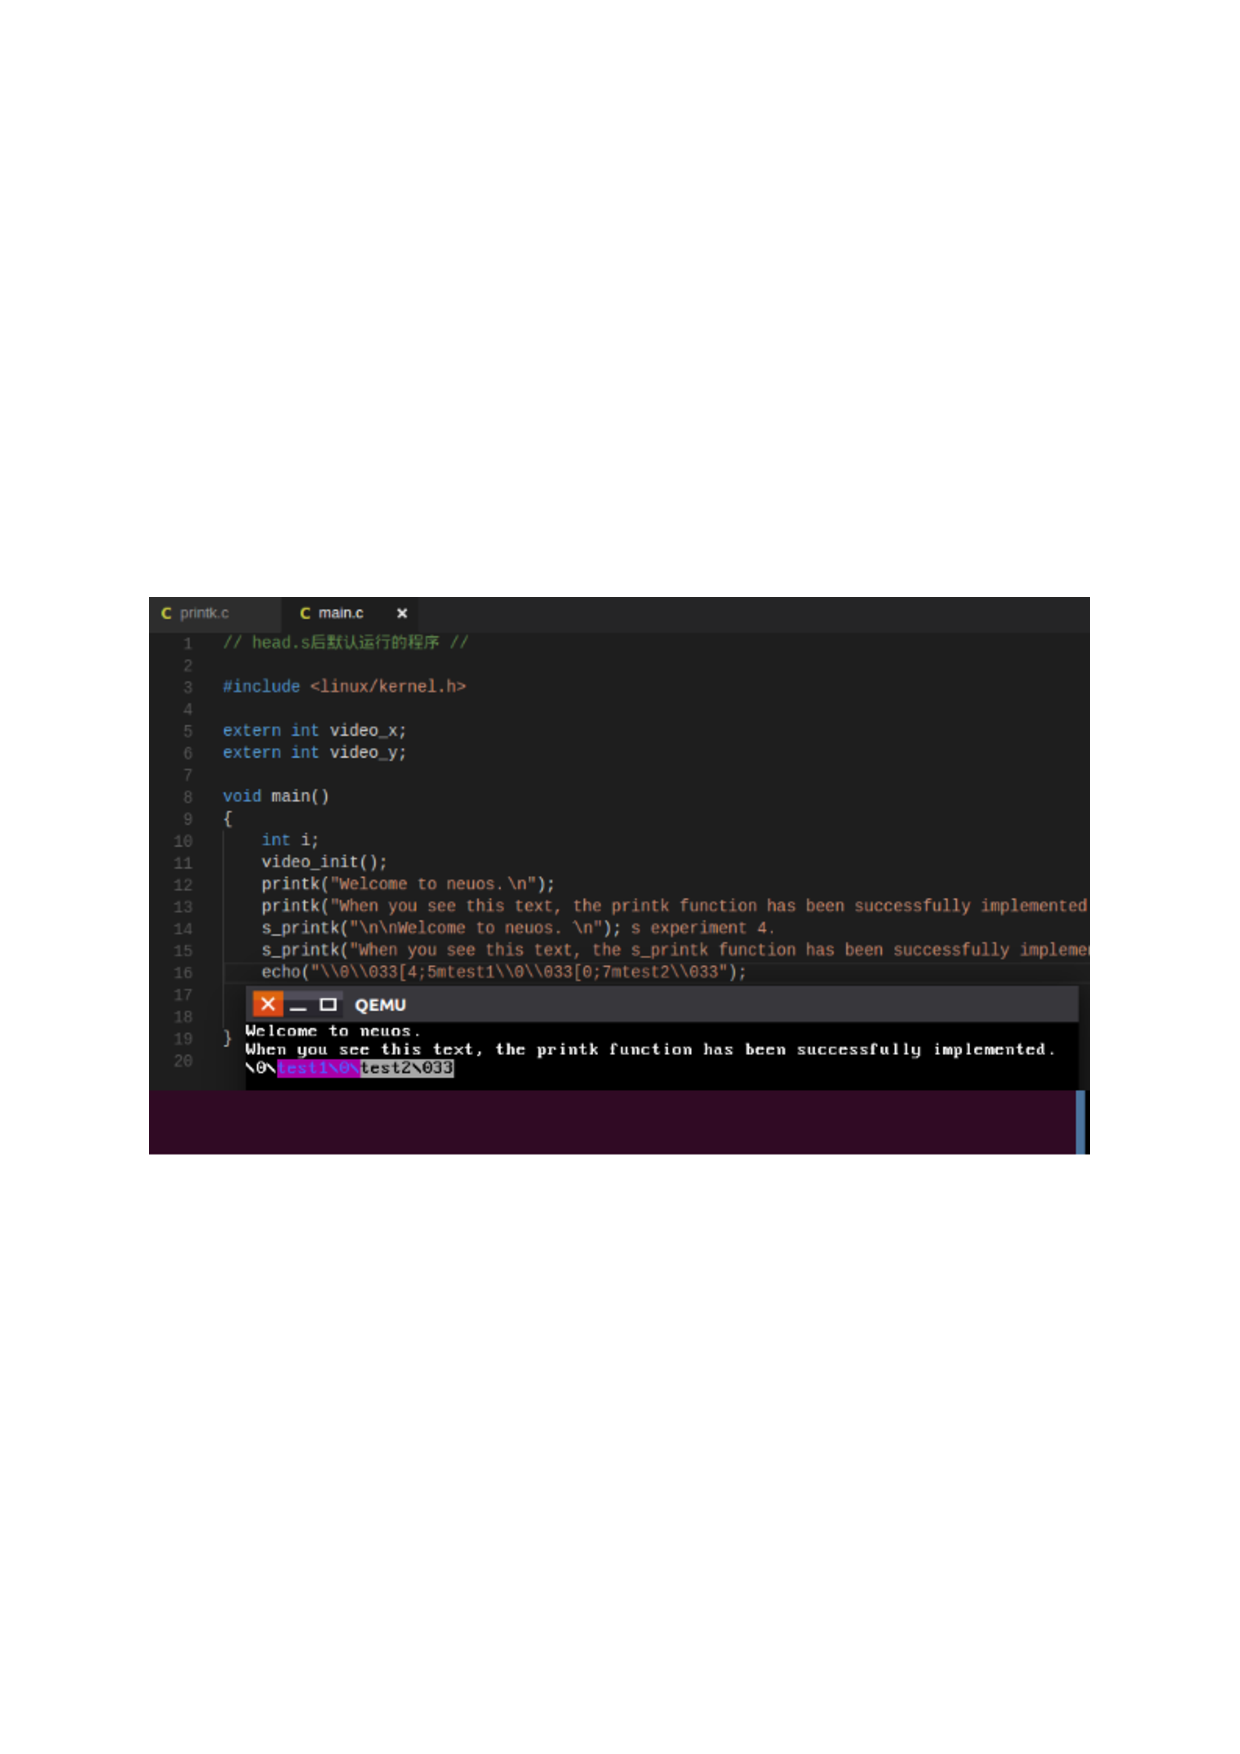
\includegraphics[width=\textwidth]{img/函数echo实现效果.pdf}
    \caption{函数 echo 实现效果}
    \label{fig:函数echo实现效果}
\end{figure}
